\documentclass[12pt, a4paper]{report}
% do not stop on errors
% \nonstopmode

\title{Accelerating agent based\\Python models}
\date{\today}
\author{Robert Kruszewski}


%\setlength\parindent{0pt}
\usepackage{tabularx, alltt, amsmath, multirow, graphicx, url, graphics, caption, natbib}
\usepackage{listings}
\usepackage{parcolumns}

\usepackage[hidelinks]{hyperref}

%Our Executive Summary
\renewcommand{\abstractname}{Abstract}

% Better looking chapters headings
\usepackage{titlesec}
\titleformat{\chapter}
  {\normalfont\LARGE\bfseries}{\thechapter}{1em}{}
\titlespacing*{\chapter}{0pt}{3.5ex plus 1ex minus .2ex}{2.3ex plus .2ex}

\begin{document}

\begin{titlepage}

\newcommand{\HRule}{\rule{\linewidth}{0.5mm}} % Defines a new command for the horizontal lines, change thickness here

\center % Center everything on the page

%----------------------------------------------------------------------------------------
%   HEADING SECTIONS
%----------------------------------------------------------------------------------------

\textsc{\large Imperial College London}\\[1.5cm] % Name of your university/college
\textsc{\large Department of Computing}\\[0.5cm] % Major heading such as course name
\textsc{\large}\\[0.5cm] % Minor heading such as course title

%----------------------------------------------------------------------------------------
%   TITLE SECTION
%----------------------------------------------------------------------------------------

\HRule \\[0.4cm]
{ \huge \bfseries Accelerating agent based\\\vspace{0.4cm}Python models}\\[0.4cm] % Title of your document
\HRule \\[1.5cm]

%----------------------------------------------------------------------------------------
%   AUTHOR SECTION
%----------------------------------------------------------------------------------------

\begin{minipage}{0.4\textwidth}
\begin{flushleft} \large
\emph{Author:}\\
Robert Kruszewski\\
\end{flushleft}
\end{minipage}
~
\begin{minipage}{0.4\textwidth}
\begin{flushright} \large
\emph{Supervisors:} \\
Dr. Anthony \textsc{Field} \\% Supervisor's Name
Dr. Michael \textsc{Lange} \\% Supervisor's Name
%Michael \textsc{Hadjiyiannis}
\end{flushright}
\end{minipage}\\[5cm]

% If you don't want a supervisor, uncomment the two lines below and remove the section above
%\Large \emph{Author:}\\
%John \textsc{Smith}\\[3cm] % Your name

%----------------------------------------------------------------------------------------
%   DATE SECTION
%----------------------------------------------------------------------------------------

{\large \today}\\[3cm] % Date, change the \today to a set date if you want to be precise

%----------------------------------------------------------------------------------------
%   LOGO SECTION
%----------------------------------------------------------------------------------------

%\includegraphics{Logo}\\[1cm] % Include a department/university logo - this will require the graphicx package

%----------------------------------------------------------------------------------------

\vfill % Fill the rest of the page with white space
\end{titlepage}
%% Ending of title page

\pagenumbering{roman}
\tableofcontents

\begin{abstract}
\begin{center}
\lbrack ABSTRACT\rbrack
\end{center}
\end{abstract}
\pagenumbering{arabic}



\chapter{Introduction}\label{ch:intro}
\begin{center}
\lbrack INTRODUCTION\rbrack
\end{center}
% We want to use Python due to widespread use in research field.
% The problem - Python (CPython) isn't truly multithreaded
%     CPython (interpreter in use) has GIL
%         other implementations would be difficult to embed in C/Fortran code base

% \section{Contributions}\label{sec:contributons}
% \begin{itemize}
%     \item Familiar syntax
%     \item Same performance as pure C
%     \item Allows for multithreading and can be deployed in real life applications
% \end{itemize}

\chapter{Modeling Plankton Ecosystems}\label{ch:bkg}

With plankton contributing about 70\% of oxygen production and
constituting most of biological production on the planet it has
become important to understand systems in which it develops and
grows. Due to its abundance it has a large impact on earth's
atmosphere, particularly regulation of carbon dioxide amounts.
Understanding beneficial and harmful effects of human's influence
on the oceans is one of the most challenging open scientific
problems. Being the fundamental element of every marine ecosystem
understanding plankton development is crucial.

Marine ecology can be understood by observations. It involves
taking measurements in specified region and computing statistical
properties in question. This process is limited with its scale
and require understanding of the context in which the measurements
re taken. On the other hand mathematical simulation involve creating
abstract representation of the environment and objects in it and
allow the underlying principles develop the ecosystem through time.
Despite the fact that our knowledge of marine ecosystems is limited
we do have good understanding of several basic processes. Therefore
methodologies that allow specifying behaviour in terms of primitive
biological equations which allow for demographic properties to emerge
from simulation are likely to be more accurate. Thus any number of
scenarios can be created and What-if? predictions can be carried out.
Naturally the accuracy of those predictions depends on correctness
of the simulation itself.

The model needs to simulate the whole ecosystem: the chemical environment,
the underlying physics principles and interaction between agents themselves
as well as environment. Those requirements lead very quickly to complex systems
that need a lot of computational power. Furthermore the simulation framework
should be general enough to accommodate changing environment; different chemical composition,
varied species and changes in physical conditions.

What remains constant between different ecosystems is the method which governs interactions
between elements and how the system develops over time irrespective of the environment
under consideration. The procedure which underpins the model is called a Metamodel\ref{sec:meta}
and is a design decision when creating simulation software.

\section{Metamodel}\label{sec:meta}
Plankton ecosystems can be classified according to the metamodels which govern
the way the plankton is aggregated. Throughout the years four metamodels have
been developed, i.e. box, field, Lagrangian ensemble (LE) and individual. They
are of increasing computational complexity and apart from LE metamodel present
completely different approach to the problem. The box metamodel is on one end
of the spectrum where the organisms are represented by average value of
properties in certain volumetric space. The individual model, however,
models every organism as a separate object thus allowing to describe the system
in terms of primitive biological equations.

\subsection{Field Metamodel}\label{subsec:field-meta}
The field metamodel uses spatial fields to describe the plankton population.
It considers the properties that the system is composed of and for each
of them constructs continuous field over the space in question. Such
treatment does not allow to model individual organisms but instead
focuses on the demographic properties of the population, i.e. what is
density of certain value at given point instead of allowing for free
interaction of organisms with the environment and each other.

Since there is no need to model each organism individually but only
each property using this metamodel lowers computational complexity
but forces modeling at higher level of the system. That is the
properties of the system and their changes in time have to be studied
and behaviour has to be extracted. While in nature the behaviour of
individual organisms lends itself to emergence of patterns in changes
of system properties.

\paragraph{Spatial Field}\label{par:field}
Spatial Field $F$ is a function of n dimensional spatial variables.
We distinguish two types of fields: scalar, where the function $F$
takes scalar values, e.g. concentration of chemical element at certain
point $(x,y)$ and vector, which takes on vector values, like
velocity of wind at location $(x,y,z)$.

Usually the measurements will be obtained as discrete set of points.
Therefore the function $F$ is obtained from finite set of
measurements $$F(x_1,y_1),\ldots,F(x_N,y_N)$$ performed at $N$ discrete
points $(x_i,y_i)$

\subsection{Individual Metamodel}\label{subsec:agent-meta}
The individual metamodel is the extreme end of the modeling spectrum.
The aim is to represent each organism in the simulation as an object
and let those interact with environment and each other. Such models
quickly become complex with due to the size of the simulated problem
and require large amount of computational power. Their emergence
was only possible due to rapidly rising computer power.

The benefit of individual based metamodels over field and box metamodels
is the ability to use primitive biological equations to represent
elements of simulation. Those equations can be obtained by observation
of individuals of desired species and does not involve analyzing
large population. As a result the model will represent the nature
more accurately and gives a possibility of accurate results and
therefore better predictions. As has been mentioned the downside
is the computational complexity.

\subsection{Lagrangian Ensemble Metamodel}\label{subsec:le-meta}
Combination of field and individual based metamodel allows for trade-off
between accuracy of the model and complexity. The Lagrangian Ensemble
metamodel uses biologically-lagrangian integration to follow the life
history of each plankter, and ensemble statistics to compute the bulk proper-
ties of whole populations. In such it behaves like individual based model
when considering single organism but at the same time uses spatial fields
to describe the properties of the population.

The Lagrangian Ensemble metamodel results in a compromise between field
and individual based approaches. As a way to achieve the flexibility
each agent in the simulation represents number of identical individuals.
The sub-population of an agent is dynamic and governed by particle
management rules. In the extreme Lagrangian Ensemble metamodel can
approximate individual based metamodel, i.e. when sub-population size is
set to 1. On the other extreme it can be used to represent field metamodel
by creating only one subpopulation. With the ability to adjust
sub-population size of agents the LE metamodel allows us to address
computational performance while limiting demographic noise.

\section{Virtual Ecology Workbench (VEW)}\label{sec:vew}
The Virtual Ecology Workbench (VEW) (shown in figure \ref{fig:VEW})
is a software suite that provides tools to make plankton ecosystem
simulations in a mid-ocean mesocosm easy. It is aimed at biological
oceanographers, thus doesn't require programming knowledge. It uses
Lagrangian Ensemble metamodel to govern the simulation. In this
metamodel the emergent demographic properties are derived from
individual based agents which in turn are described
using primitive biological equations. Each simulation created
by VEW is globally stable, adjusts to attractor that is independent
of initial condition \cite{Woods2005}. Therefore such simulations
are useful for What-if? Prediction.

\begin{figure}[ht!]
  \begin{center}
    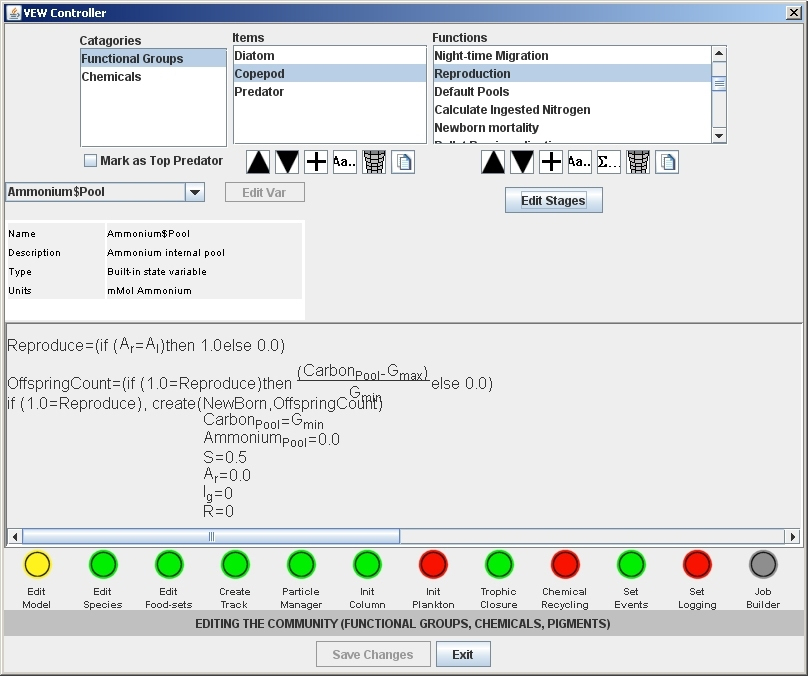
\includegraphics[width=0.7\textwidth,natwidth=800,natheight=707]{../vew2007-10.jpg}
    \caption{Virtual Ecology Workbench provides a complete suite of tools to model
    ocean ecosystems}
    \label{fig:VEW}
  \end{center}
\end{figure}

Virtual Ecology Workbench enables users to create simulation using
phenotypic equations in form familiar to them. It automatically
generates necessary code to represent environment and species
specified by user. The Lagrangian Ensemble metamodel
provides good trade-off of computational complexity and accuracy.
The metamodel computes emergent properties, the demography
of species population and biofeedback between agents and environment.
The simulation describes life history of every individual plankter
in the ecosystem to make it possible. Each agent in the simulation
behaves like a population of multiple identical plankters. Each
plankter in the ecosystem is contained in one of those agents.
Simulation created by VEW employ splitting and merging techniques
to ensure that that population is adequately represented and
that sampling is accurate where each agent can be subdivided into
multiple or two agents can be merged together. Therefore the
total number of agents can always stay within boundaries
defined by the user.

\subsection{Environment}\label{para:1d-phys}
\begin{figure}[ht!]
  \begin{center}
    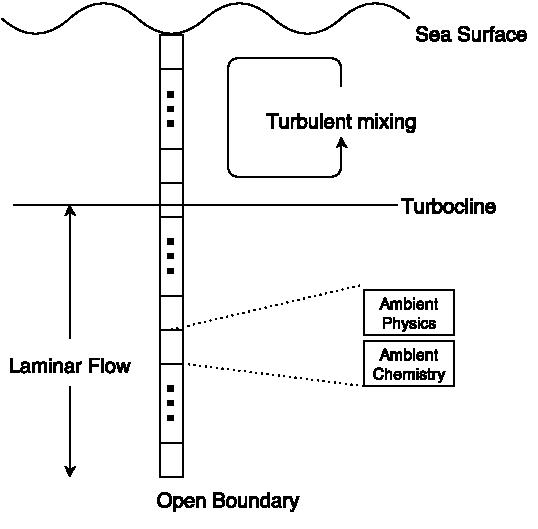
\includegraphics[width=0.6\textwidth,natwidth=473,natheight=466]{../env-diagram.pdf}
    \caption{Physical environment in which VEW carries out the simulation}
    \label{fig:env}
  \end{center}
\end{figure}

Figure \ref{fig:env} illustrates the environment that is employed by VEW
to carry out its simulation. The physical environment as defined by Woods \cite{Woods2005}
is a one-dimensional water column for us in open ocean where water depth exceeds 1km.
The vertical axis extends from the sea surface to depth of, typically, 0.5km.
VEW allows for the column to drift with ocean currents or be hoisted in place.
Solar and infra-red radiation, sensible and latent heat, water vapour
and other gases pass through the upper boundary while the lower is open
and allows detritus to sink through to the deeper parts of the ocean.
The physical model makes an assumption that even though the
water can flow freely through side walls of the environment it produces
zero flux divergence in every ecosystem property at all depths.

There are two reasons why approximation through one-dimensional model is
acceptable and will produce good results. First of all, the plankton being
modeled lives mostly in seasonal boundary layer of the ocean which has structure
controlled mostly by vertical fluxes. Secondly, the horizontal correlation
scale of the environment variables is typically two orders of magnitude greater
than the vertical scale. Planktons cannot usefully change their ambient environment
by swimming horizontally. However, many species of plankton do change their
ambient environment by swimming horizontally. This one-dimensional model is a very
good first approximation. It has to be noted though that the principal source
of errors arises from the neglect of mesoscale turbulence which is mostly correlated
in horizontal scale. Simulation of plankton ecosystems with mesoscale turbulence
requires three dimensional version of LE metamodel. In work by Lange \cite{FluidityVEW}
the author shows how to integrate VEW generated models into general computational
fluid dynamics framework and demonstrates that the resulting system adjusts to
similar attractors as one-dimensional version.

\subsection{Functional Groups}\label{subsec:fg}

At the core of Lagrangian Ensemble modeling there are functional groups (FG).
Functional groups are the highest level grouping in marine biodiversity
parameter space. It defines set of variables that represent agent's internal
biochemical state. Furthermore it is used to define the set of phenotypic
equations that govern physiology and behaviour which are used to advance
agent to next state in time.

\begin{figure}[ht!]
  \centering
  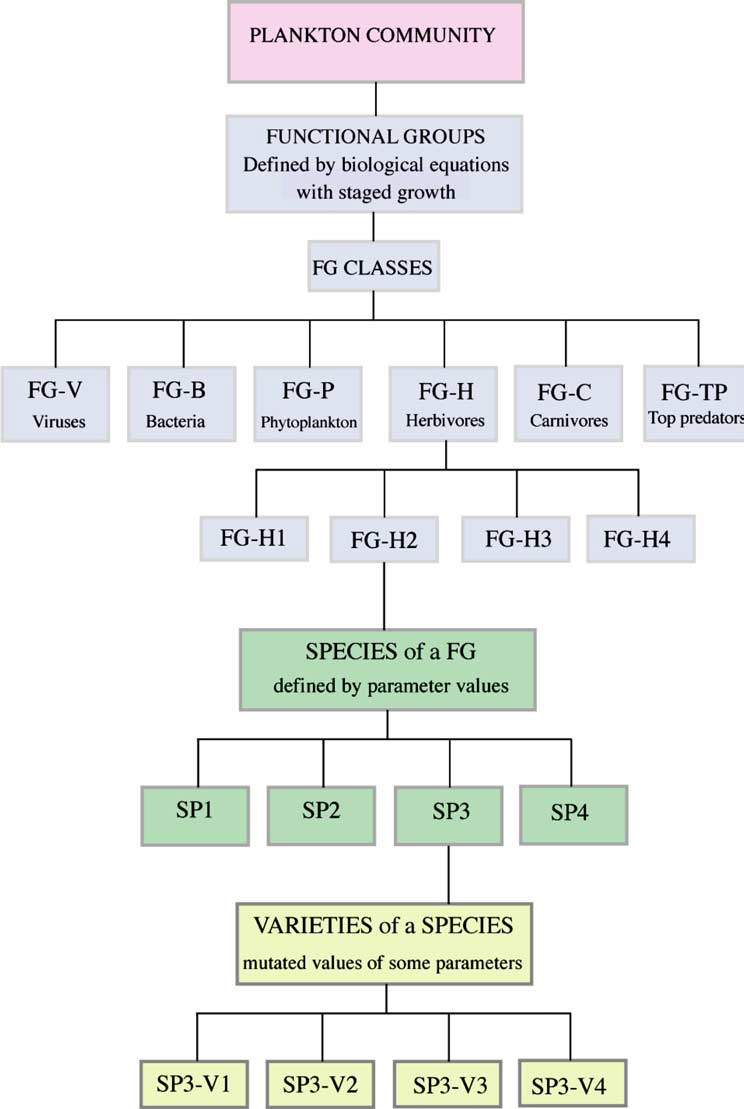
\includegraphics[width=0.7\textwidth,natwidth=744,natheight=1109]{../fg.jpg}
  \caption{Plankton community according to Woods \cite{Woods2005}
    with functional groups, species and varieties}
  \label{fig:fg}
\end{figure}

Figure \ref{fig:fg} shows grouping hierarchy of ecosystem modeling
objects. The plankton community in simulation consists of multiple functional
groups. Each of communities may be later subdivided into species. In case of
LE modeling species define parameter set for enclosing functional group set of
equations. Through parameter mutation we can achieve multiple varieties of
species. Going further down each species can be subdivided into traits.
Traits allow to factor in ecological adaptation in resource competition models.
As such traits are a way to incorporate evolution into ecosystem models
which is a current trend in modeling \cite{Clark20113823}.

The major difference in Lagrangian Ensemble model as proposed by Woods
\cite{Woods2005} is the ability to capture life-cycle of individual. This
feature is impossible to emulate in population-based approaches. As a
consequence each agent can have particular stage associated with it. Agent's
stage defines physiological processes currently active in subpopulation hence,
the phenotypic equations that are being used at particular timestep. The LE
allows for incorporation of growth, dormant stages and over-wintering as
seen in nature. The metamodel acknowledges the fact that physiological
behaviours of individuals may change over time and thus should be represented
in the model. Different growth stages constitute important source of intra-population
variability in ecosystem modeling.

\subsection{Model Specification - Planktonica}\label{subsec:planktonica}
The way in which model is specified in Virtual Ecology Workbench is through
Planktonica \cite{Planktonica}. Planktonica is a modelling language for
designing plankton. Arbitrary chemicals, with different action spectra to
represent pigmentation, can be used. Planktonica allows for encapsulation of
metamodel which describes basic rules in which simulation is carried out
like the definition of particle, the way the may interact and definition
of environment.

Planktonica creates the simulation code from the high level description
provided by the user. Thus it does not require programming knowledge.
The descriptions provided are transformed to an XML model which is
further enriched by later stages of VEW pipeline. Finally Planktonica
itself generates the code required to run the simulation for specified
model. Figure~\ref{fig:planktonica} Illustrates how the parts of the system
communicate together.

\begin{figure}[ht!]
  \centering
  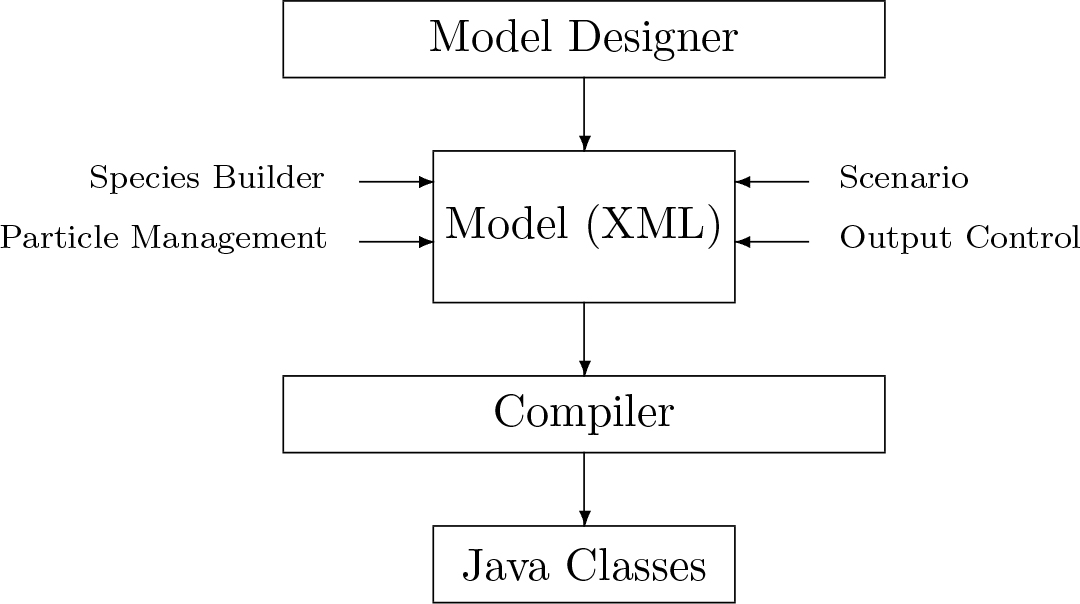
\includegraphics[width=0.7\textwidth,natwidth=1080,natheight=604]{../planktonica.jpg}
  \caption{Schematic working of Planktonica as described by Hinsley \cite{Planktonica}}
  \label{fig:planktonica}
\end{figure}

\subsection{Agents}\label{subsec:agents}
Lagrangian Ensemble metamodel has the ability to represent
multiple organism from same subpopulation into one agent.
Therefore plankton in the simulation can be described in
terms of primitive biological equations which are
observable in laboratory experiments. Instead of defining
each elements behaviour separately the LE metamodel uses
functional groups, species and stages to define set of
variables that govern its state and transitions.
Due to independence of agent updates from state all of the
biochemical processes can be defined once for any species
in particular stage. This is to the contrary to field models
where each property changes differently depending on a location
on a fixed mesh\cite{Woods200543}. Furthermore agents are able to
nondeterministically change their internal biological
state via stage transitions. In order to manage
those extra care has to be taken in particle management.

\subsection{Physics - Particle Management}\label{subsec:physics}
Due to individual based nature agent based model require a sampling
strategy to represent large number of plankters per cubic metre in the
ocean while keeping the problem computational feasible. This is achieved
in Lagrangian Ensemble metamodel via number-based up-scaling mechanism,
i.e. single agent represents multiple identical individuals. In order
to be able to compute demography of the population realistically
every individual has to occur in one of the agents present in the
environment. Due to the fact that number of individuals may change
significantly during particular time step. Therefore agent accounting
method is necessary to keep the number of agents during simulation
in desired range.

Restriction on number of agents are enforced by Particle Management.
The manager provides the trade-off between accuracy and speed of the
simulation. In order to enforce bounds specified by the user
the agent population is re-sampled using a continuous split/combine
algorithm. The number of agents is increased in a given region
by splitting the largest of agents in the set evenly until
the minimum threshold value is surpassed. Converse happens when
merging. The smallest agent in region are merged in pairs of two
and resulting agent has the weighted average of variables from source
set.

\begin{figure}[ht!]
  \begin{center}
    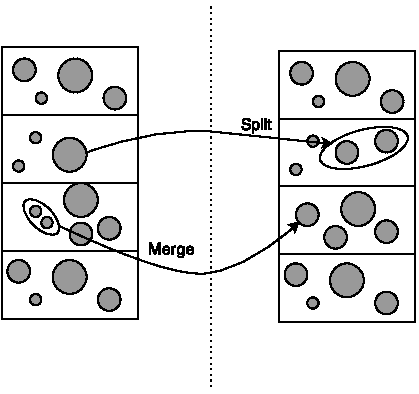
\includegraphics[width=0.4\textwidth,natwidth=366,natheight=342]{../Split_merge.pdf}
    \caption{Example of Split/Merge in action}
    \label{fig:split-merge}
  \end{center}
\end{figure}

This method is illustrated in Figure \ref{fig:split-merge},
where a target density of four agents per level is requested.

\section{Fluidity}\label{sec:fluidity}
The biggest disadvantage of models generated by VEW is the 1D environment.
It does not allow for horizontal movement and according to authors
``serves as a good first approximation'' \cite{Woods2005}. It is still an approximation.

In work done by Lange \cite{FluidityVEW} Fluidity, general-purpose
computational fluid dynamics software, has been adapted to incorporate
ocean modelling. Fluidity \cite{Piggot2008,fluidity} is capable of
solving Navier-Stokes equations and accompanying field equations on
arbitrary unstructured finite element meshes. The computation is
parallelised using MPI and uses adaptive remeshing to optimize the
underlying mesh structure at runtime. Therefore achieving computational
efficiency and focus on regions of interests. The resulting Fluidity-ICOM
provides ocean model capable of sub-grid scale parametrization to model
turbulent mixing as well as embedding of plankton biochemistry.

Fluidity is highly configurable via graphical user interface tool Diamond
which comprises larger scheme-driven description library Spud\cite{ham2009spud}.
Using the tool users are able to define properties to be computed during the simulation.
Fluidity has three types of fields \cite{fluidity}:

\begin{itemize}
  \item Prognostic fields are computed through solving partial different equations.
    User can specify discretisation used during solve phase as well as initial and boundary
    conditions via Diamond.
  \item Diagnostic fields are computed from other fields without solving a
    partial differential equation.
  \item Prescribed fields are defined by external sources. They can encapsulate a constant
    or a user defined function which can, i.e. be used to derive environment condition
\end{itemize}

\subsection{3D Particle Management - Computational Fluid Dynamics}\label{subsec:3d-pm}
The key motivation for using Fluidity to model the physical environment
is the ability to introduce individual based plankton simulations in three
dimensional setting. With 3D meshes the impact of mesoscale turbulence,
only possible with turbulent ocean dynamics, on plankton simulations
can be investigated. In order to ensure correctness of the simulation
the interplay between ocean dynamics and ecological factors of marine
plankton ecosystem the ocean model has to be capable of resolving
turbulent flows at varying scales and resolutions.

VEW based models do not resolve turbulent nutrient dissipation within
surface mixed layer but enforces it. Fluidity has inherently different
model where it solves advection-diffusion equation with numerical eddy
diffusivity to achieve turbulent nutrient dissipation.
VEW generated simulation rely heavily on accurate convection based
cycle of mixed layer deepening. The key challenge is to integrate
mixed layer depth model used in VEW and Fluidity's advection-diffusion
equations. In order to achieve the desired effect K-profile parametrisation
is used alongside VEW's MLD model.

\paragraph{Adaptive Remeshing}\label{para:remesh}
What makes Fluidity attractive for large scale simulations is its ability
to dynamically adapt the underlying mesh at runtime. The process minimises
discretisation errors and focuses resolution on regions of particular interest.
The adaptive mesh refinement uses anisotropic metric tensor field which
describes desired geometric properties necessary to minimise interpolation error.
The metric tensor can be formed from multiple fields and is computed using
Hessian of the fields under consideration. Therefore Fluidity's adaptive
mesh will have higher resolution in areas of steep gradients and coarser
in regions with smooth transitions.
From point of view of ocean modelling the ratio between horizontal
and vertical dimensions should be high. Particularly is meso-scale processes
are to be resolved. Fluidity has the ability to decouple vertical
and horizontal adaptation steps resulting in columnar mesh where elements
are aligned vertically and extruded from underlying horizontal two-dimensional mesh.
The vertical resolution is adapted independently of horizontal and allows
for linking between all columns to form a layered mesh.

\subsection{Model Specification - Python}\label{subsec:model-spec-py}

Python is used throughout Fluidity-ICOM implementation to provide flexible
interface which serves as a further customisation to configuration options.
The provided Python code is used to prescribe and manipulate field data.
Fluidity employs CPython via it's C-API to allow on the fly computation
of user provided options.

Diamond is used in Fluidity to provide easy way to modify large
configuration files. Python code can be conveniently embedded via its
interface.
\begin{figure}[ht!]
  \begin{center}
    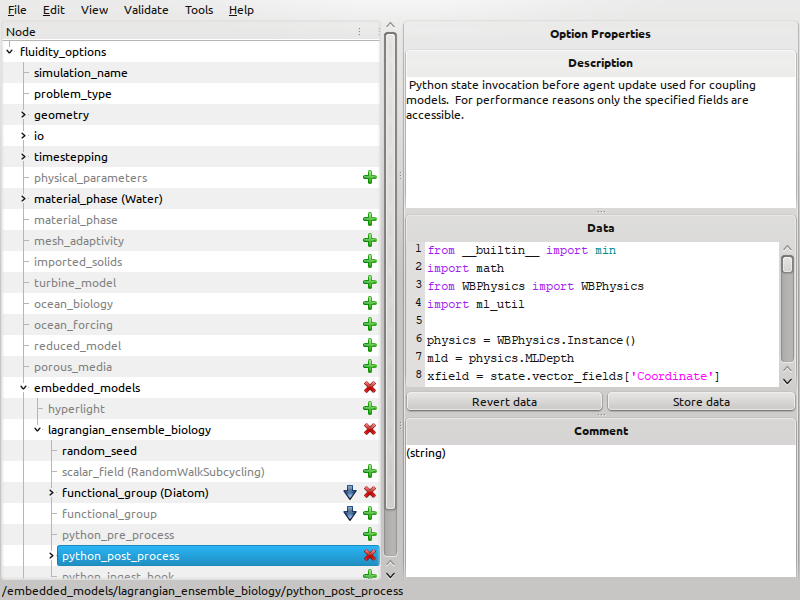
\includegraphics[width=0.6\textwidth,natwidth=800,natheight=600]{../diamond.png}
    \caption{Diamond - Fluidity's configuration creator}
    \label{fig:diamond}
  \end{center}
\end{figure}

The embedded interpreter is used two fold
\begin{itemize}
  \item Space and time-varying field data - Space and time-varying field
data may be entered as a Python function to define prescribed fields
or enter the initial condition of a prognostic field.
  \item Python State - Fluidity also provides access to its internal state and
field data via the Python State interface. This interface allows the
user to define custom diagnostic algorithms, where the nodal values
of a diagnostic field are set by the user-defined Python function.
Furthermore, this interface may also be used to define Eulerian ecology
models by setting the relevant source and absorption terms of the
prognostic fields representing the ecosystem components.
\end{itemize}

\chapter{LERM}\label{ch:lerm-toy}
Throughout this thesis the model employed is based on
Lagrangian Ensemble Recruitment Model (LERM) as first designed
by Sinerchia et al. \cite{FisheriesRecruitment}. LERM is a
fisheries recruitment model that uses four trophic levels to
model the effects of predation and competition on squid recruitment.

\section{Simple LERM}\label{sec:lerm-simp}
While the original model provides realistic example in order
to focus on performance aspects of simulation as simplified version
is used. Thus only Diatoms, plant-based plankters, are present
as agents. Top level predators as well as Copepods (animal-based plankton)
are ignored in this version of the model. There is no predation
between agents, hence there is no need to simulate ingestion.
While those restrictions focus biological environment we will also
disregard bio-optical feedback and read physical environment
information: temperature, visible irradiance, level of turbocline layer and depth of water column, from files
generated by full Java based VEW simulation.

\chapter{Parallelisation}\label{ch:para}

\section{OpenMPI}\label{subsec:openmpi}
Message Passing Interface is a way of distributing computation
amongst several machines via network connection. Each of the
machines (nodes) in the system is able to issue and receive
messages which are a mean to spread the workload.
OpenMPI is a result of merger of several MPI libraries, like
LAM/MPI, LA-MPI, and FT-MPI. It aims to standardise the implementation
and improve interoperability. Thus reducing the burden on
end users and increasing adoption. It provides production-quality
MPI-2 implementation. Currently OpenMPI is de-facto the MPI
library. Apart from being a quality MPI implementation is to
facilitate third-party research and creation of independent
add-ons.

\section{OpenMP}\label{subsec:openmp}
While OpenMPI focuses on distributing workload amongst different
machines OpenMP is used to distribute tasks in one machine amongst
several cores. Due to it's memory oriented nature there's a significant
penalty incurred when operating across different cache domains.
OpenMP aims to provide compiler directives, library routines, and environment variables
for shared-memory parallelism in C, C++ and Fortran programs.

In contrast to other multithreading approaches OpenMP provides high
abstraction level thus enabling portability. The portability of OpenMP directives
is ensured by runtime library which is platform dependent part of implementation.
The directives it introduces focus on single program multiple data
(SPMD) constructs, tasks, worksharing and synchronisation.
Furthermore the library provides means of sharing and privatizing
data across threads.

OpenMP only covers user-directed parallelization, where programmer explicitly
states actions which are to be taken by compiler to make program parallel at runtime
Any implementation is not required to check for data dependencies, data conflicts,
race conditions, or deadlocks which may occur in multithread programs.
The specification does not cover compiler-generated automatic parallelization and
directives to the compiler to assist such parallelization.

Since OpenMP is tightly integrated with the compiler it is non-trivial to
understand types of transformation that are performed to make program parallel.
Listing \ref{list:openmp-dir} and \ref{list:openmp-run} shows one of the transformation that is performed.

\begin{lstlisting}[caption=OpenMP directives,frame=tlrb,label=list:openmp-dir,language=c]{OpenMP directives}
#include <omp.h>
void main() {
  #pragma omp parallel
  {
    int ID = omp_get_thread_num();
    printf(“Hello world(%d)”, ID);
  }
}
\end{lstlisting}

\begin{lstlisting}[caption=OpenMP runtime,frame=tlrb,label=list:openmp-run,language=c]{OpenMP runtime}
void __ompregion_main1(...) {
  int ID = ompc_get_thread_num();
  printf(“Hello world(%d)”,ID);
} /* end of ompregion_main1*/

void main() {
  ...
  __ompc_fork(&__ompregion_main1,...);
  ...
}
\end{lstlisting}

\section{Isoefficiency}\label{sec:isoeff}
Isoefficiency is a measure of how in relation to growth in number of parallel execution units the working set has to grow in order to maintain same efficiency of the system. In general with growing working set size given constant number of processors the efficiency increases while the inverse happens when working set size is constant and number of parallel execution units increases.
\begin{equation}\label{eq:isoeff} W = \dfrac{E}{1-E}T_o(W,p) \end{equation}
\ref{eq:isoeff} describes relation between working set size and efficiency for parallel system as defined in \cite{grama2003introduction}.
For any scalable system efficiency can be maintained at a fixed value if the ratio \[\dfrac{T_o}{W}\] is kept at a constant value.
Let \[K = \dfrac{E}{1-E}\] be a constant depending on the efficiency to be maintained. The we have
\begin{equation}\label{eq:isoconst} W = KT_o(W,p) \end{equation} Knowing properties for a particular system we can obtain value of W
as a function of p which dictates the rate at which working set size has to grow in order to maintain fixed efficiency.

\section{Python Multithreading}\label{subsec:mult-py}

\subsection{Global Interpreter Lock (GIL)}\label{subsec:GIL}

% \chapter{Embedding Python in C applications}\label{ch:python-embedding}

% \section{Python C-API}\label{sec:python-capi}

% \section{Cython}\label{sec:cython}

% \subsection{Avoiding GIL}\label{subsec:avoiding-gil}

% \begin{figure}[t]
%   \begin{center}
%     % \showthe\columnwidth % Use this to determine the width of the figure.
%     \includegraphics[width=\columnwidth]{fig1.eps}
%     \caption{\label{fig:sin_cos} Plot of the sine and cosine functions.}
%   \end{center}
% \end{figure}

% To add something to the bibliography, look for the "import into BibTex" thingy on google scholar, and add the stuff into refs.bib.
\bibliographystyle{plain} \bibliography{References}

\end{document}
